\documentclass[10pt]{beamer}

%load any additional packages

\usepackage[UKenglish]{babel}
\usepackage[utf8]{inputenc} % so we can input characters with accents (e.g. ő)

\usepackage{statsbeamer}
\usepackage{multirow,booktabs}%pacotes para tabelas
\usepackage{subcaption}
\usepackage[font=footnotesize,skip=2pt]{caption}
%\captionsetup[table]{skip=2pt}
\usepackage{ragged2e}
\usepackage{hyperref}
\usepackage{tikz}
\usetikzlibrary{arrows.meta}
\tikzset{%
  >={Latex[width=2mm,length=2mm]},
  % Specifications for style of nodes:
            base/.style = {rectangle, rounded corners, draw=black,
                           minimum width=4cm, minimum height=1cm,
                           text centered, font=\sffamily},
  activityStarts/.style = {base, fill=oxfordblue!30},
       startstop/.style = {base, fill=oxfordblue!30},
    activityRuns/.style = {base, fill=oxfordblue!30},
         process/.style = {base, minimum width=2.5cm, fill=orange!15},
}

\usepackage{graphicx} % ease graphics management
\graphicspath{{figs/}} % define folder with images
\usefonttheme{serif} % change font to allow \textbf{}
\usepackage{charter} % Nicer fonts

\usepackage{cancel}
\usepackage{amsmath,amsthm,amssymb} % for math equations

\usepackage[numbers]{natbib} % richer citation
\usepackage{breakcites} % avoid overfull hbox for long cites

\usepackage{algorithm,algorithmic}                                          % Pseudo-code environment
\usepackage{amsmath,amsfonts,amsthm,amssymb,bm,mathdots,mathtools,bigints}  % Math packages

\usepackage{caption}                        % Tools for customizing the \caption{} command
\usepackage{subcaption}						% Environment to create subcaptions

\captionsetup{singlelinecheck = false, format= hang, justification=raggedright, font=footnotesize, labelsep=space} % ABNT Format for Caption
%% Information (author, title, etc.) %%

\title[Short Title]{% short title for footer
    Separable Least-Mean Squares Beamforming 
    \vspace{0.5cm}
}

\author{Kenneth B. dos A. Benício}

\institute{
        \textit{Department of Teleinformatics Engineering}\\
        \textit{Federal University of Ceará}
        \vspace{0.5cm}
}
\date[Fortaleza, 2021]{% short date for footer
    Fortaleza, 2021
}


%% Content of slides %%
\begin{document}

%% Title slide
{
    \setbeamertemplate{footline}{}
    \setbeamertemplate{headline}{}
    \setbeamercolor{background canvas}{bg=oxfordblue}
    \maketitle
}


%% Contents slide
 \begin{frame}
 \frametitle{Outline}
 \tableofcontents
 \end{frame}

%% Including the slides
\setbeamercovered{transparent}

%% Problem Statement
\begin{frame}{Problem Statement}
    \begin{block}{Objectives}
        \begin{enumerate}
            \item Recover a desired source signal by employing a large antenna array following an Uniform Rectangular Array (URA).
            \item Use spatial filter (beamforming) and optimize it according to the Mean square error (MSE) criterion.
            \item Solve the problem of slow convergence presented at LMS and NLMS algorithms.
        \end{enumerate}
    \end{block}
    \begin{block}{How to do so?}
        \begin{enumerate}
            \item Exploit URA separability to reduce the convergence time of the problem.
            \item Implementing a beamforming filter of the form $\mathbf{w} = \mathbf{w}_{v} \otimes \mathbf{w}_{h}$, with $\mathbf{w}_{h} \in \mathbb{C}^{N_{h}}$ and $\mathbf{w}_{v} \in \mathbb{C}^{N_{v}}$ and $N = N_{h} N_{v}$.
        \end{enumerate}
    \end{block}    
\end{frame}

%% System Model
\section{System Model}
\begin{frame}[allowframebreaks]
    \frametitle{\insertsection}
    \begin{itemize}
        \item The received signal model follows a geometric channel
            \begin{align}
                \boldsymbol{x}[k] = \sum^{R}_{r = 1} \boldsymbol{a}(p_{r},q_{r}) s_{r}[k] + \boldsymbol{b}[k] = \boldsymbol{A} \boldsymbol{s}[k] + \boldsymbol{b}[k],
            \end{align}
        \item The vector $\boldsymbol{a}(p_{r},q_{r})$ represents an Uniform Rectangular Array (URA)
            \begin{align}
                \boldsymbol{a}(p_{r},q_{r}) = \boldsymbol{a}_{v}(q_{r}) \otimes \boldsymbol{a}_{h}(p_{r})
            \end{align}
    \end{itemize}
    \begin{figure}
        \centering 
        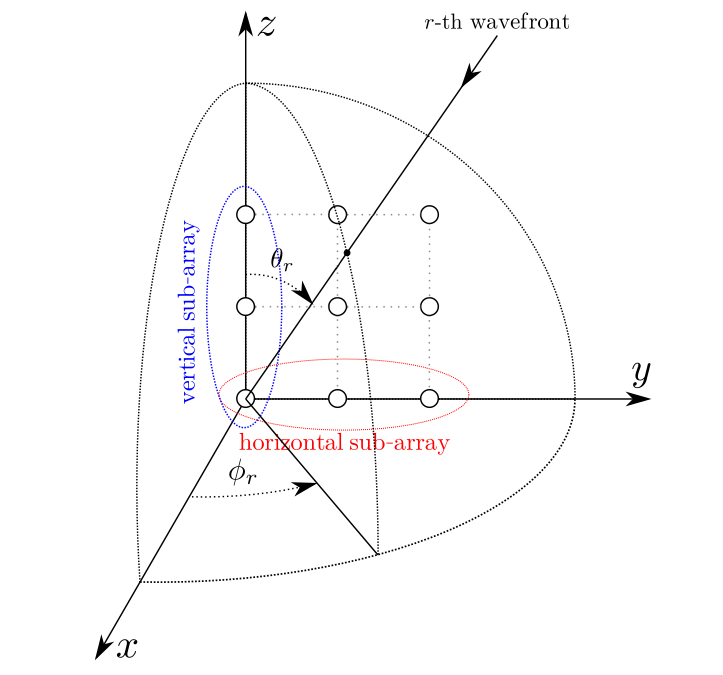
\includegraphics[width=0.70\linewidth]{ura.png}
        \caption{Unifor Rectangular Array (URA) with $3 \times 3$ elements from \cite{ribeiroseparable}.}
        \label{fig:ura} 
    \end{figure}
\end{frame}

%% Beamforming Methods
\section{Beamforming Methods}
\begin{frame}[allowframebreaks]
    \frametitle{\insertsection}
    \begin{itemize}
        \item Filter Problem 
            \begin{align}
                \mathbb{E}\{ (s_{d}[k] - \boldsymbol{w}^{\text{H}} \boldsymbol{x}[k] )^{2} \} = 0
            \end{align}
        \item Classic Wiener Filter
            \begin{align}
                \boldsymbol{w}_{\text{opt}} = \boldsymbol{R}^{-1}_{x} \boldsymbol{p}_{xs},   
            \end{align}
        \item NLMS Adaptative Filter
            \begin{align}
                y[k] &= \boldsymbol{w}^{\text{H}} \boldsymbol{x}[k], \\
                \boldsymbol{w}[k+1] &= \boldsymbol{w}[k] + \frac{\mu}{\gamma + \boldsymbol{x}^{\text{T}}[k] \boldsymbol{x}[k]} \boldsymbol{x}[k] e^{*}[k]
            \end{align}
        \item Tensor Filters
            \begin{align}
                y[k] = \left(\boldsymbol{w}_{v} \otimes \boldsymbol{w}_{h} \right)^{\text{H}} \boldsymbol{x}[k]
            \end{align}
    \end{itemize}
    \framebreak
    \begin{figure}
        \centering 
        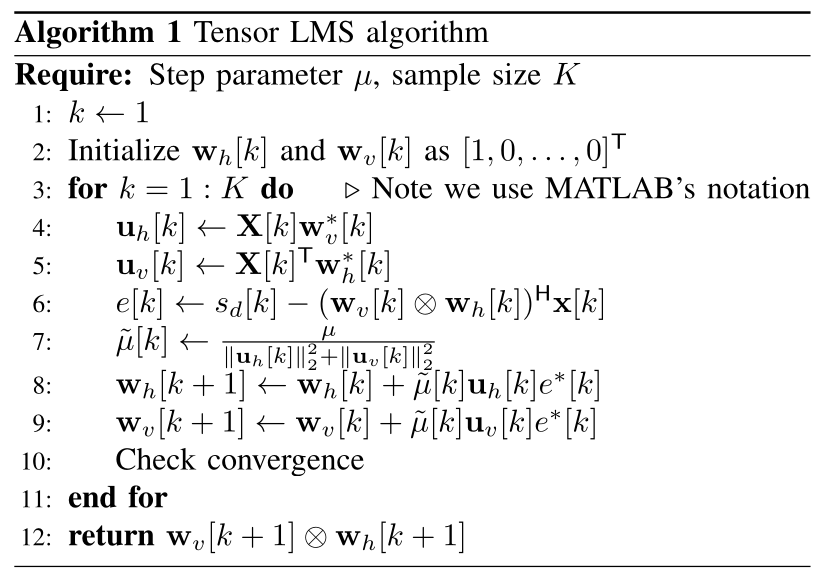
\includegraphics[width=0.90\linewidth]{tlms.png}
        \caption{TLMS algorithm from \cite{ribeiroseparable}.}
        \label{fig:lms_alg} 
    \end{figure}
    \begin{figure}
        \centering
        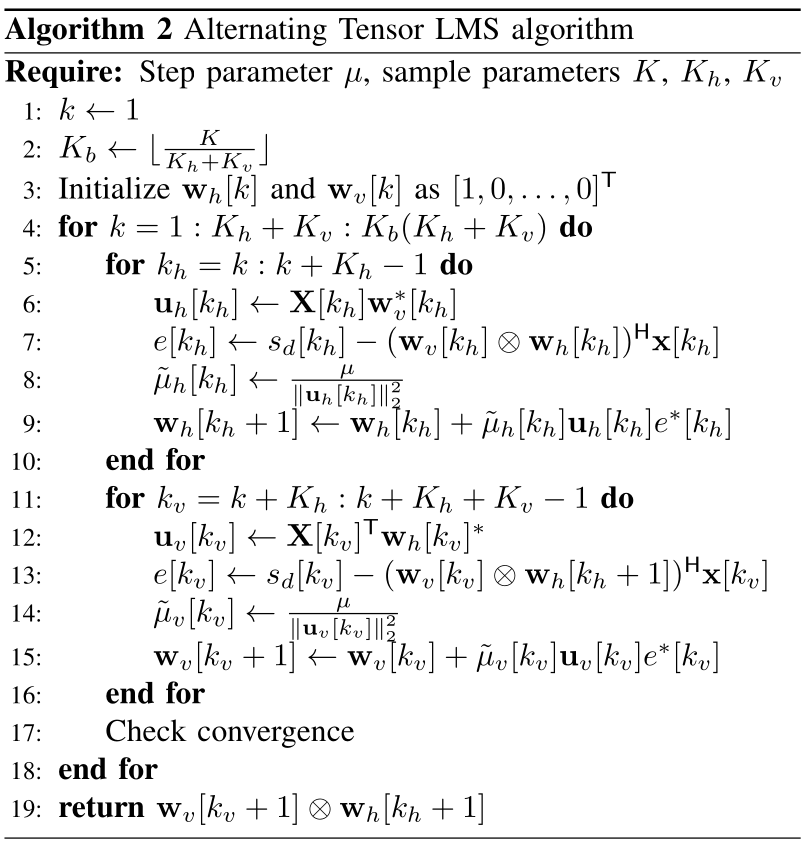
\includegraphics[width=0.60\linewidth]{atlms.png}
        \caption{ATLMS algorithm from \cite{ribeiroseparable}.}
        \label{fig:atlms_alg} 
    \end{figure}
    \begin{block}{Convergence and Computational Complexity}
        \begin{itemize}
            \justifying
            \item The convergence for TLMS in MSE is
            
                \begin{align}
                    0 < \mu < \frac{2}{\left|\left|\boldsymbol{u}_{h}[k]\right|\right|^{2}_{2} + \left|\left|\boldsymbol{u}_{v}[k]\right|\right|^{2}_{2}}
                \end{align}
            
            \item The convergence for ATLMS in MSE is
            
                \begin{align}
                    0 < \mu < \frac{2}{\left|\left|\boldsymbol{u}_{i}[k]\right|\right|^{2}_{2}}, i \in \{h,v\},
                \end{align}
            
            \item TLMS and ATLMS has a computational complexity of $O(N_{h} + N_{v})$ and NLMS of $O(N)$. Since all the methods are linear in complexity
            the most important aspect that we must observe is the convergence rate.

        \end{itemize}
    \end{block}
\end{frame}

%% Numerical Results
\section{Numerical Results}
\begin{frame}
    \frametitle{Simulation Scenario}
    \begin{block}{Parameters}
        \begin{itemize}
            
            \item It was considered an URA of $4 \times 4$ antennas with $R = 4$ multipaths and QPSK information signals.
            
            \item The SNR was defined as $\text{SNR} = 1/\sigma^{2}_{b}$.

            \item We set as figure of merit the sample Mean Square Error (MSE) defined and calculated over $K = 10000$ samples
            
                \begin{align}
                    \text{MSE}(\boldsymbol{w}) = \frac{1}{K} \sum^{K}_{k = 1} \left|\left| s_{d}[k] - \boldsymbol{w}^{\text{H}} \boldsymbol{x}[k] \right|\right|^{2},
                \end{align}

        \end{itemize}
    \end{block}
\end{frame}

\begin{frame}
    \frametitle{NLMS MSE Curve}
    \begin{figure}
        \centering
        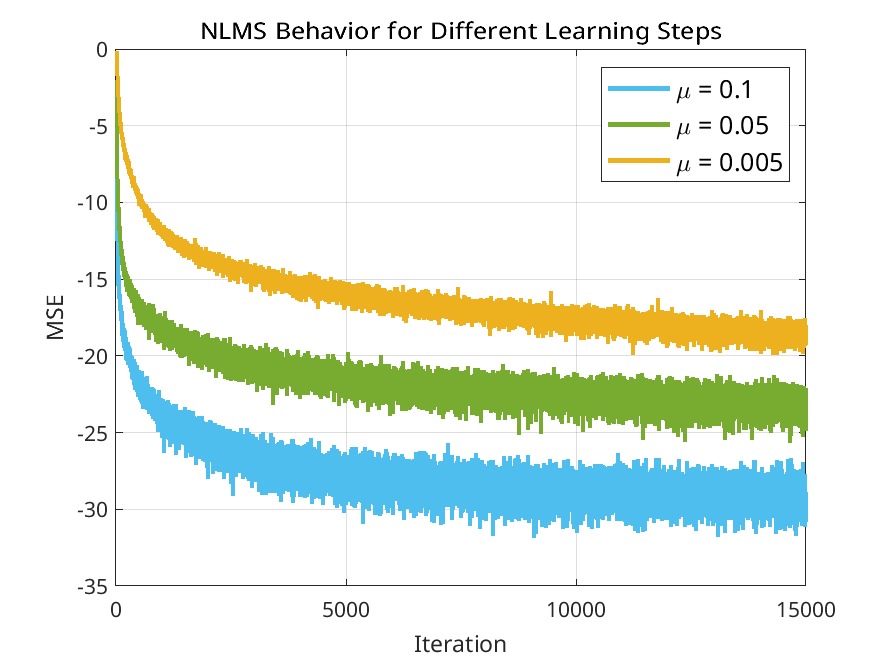
\includegraphics[width=0.90\linewidth]{nlms_mse.png}
        \caption{Monter Carlo Experiment with 2500 runs for NLMS algorithm.}
        \label{fig:nlms} 
    \end{figure}
\end{frame}

\begin{frame}
    \frametitle{TLMS MSE Curve}
    \begin{figure}
        \centering
        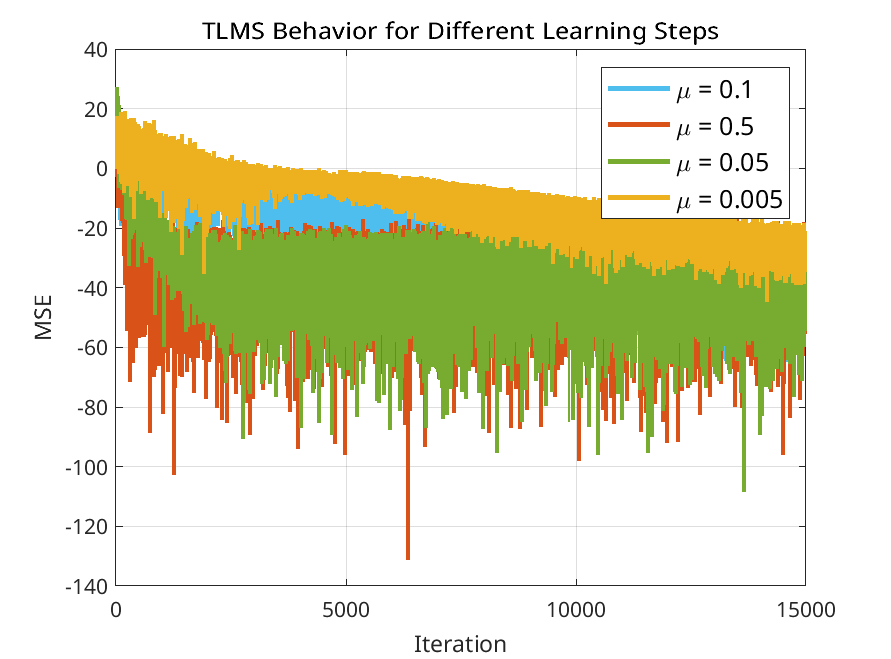
\includegraphics[width=0.90\linewidth]{tlms_mse.png}
        \caption{Monter Carlo Experiment with 2500 runs for LMS algorithm.}
        \label{fig:tlms} 
    \end{figure}
\end{frame}

\begin{frame}
    \frametitle{ATLMS MSE Curve}
    \begin{figure}
        \centering
        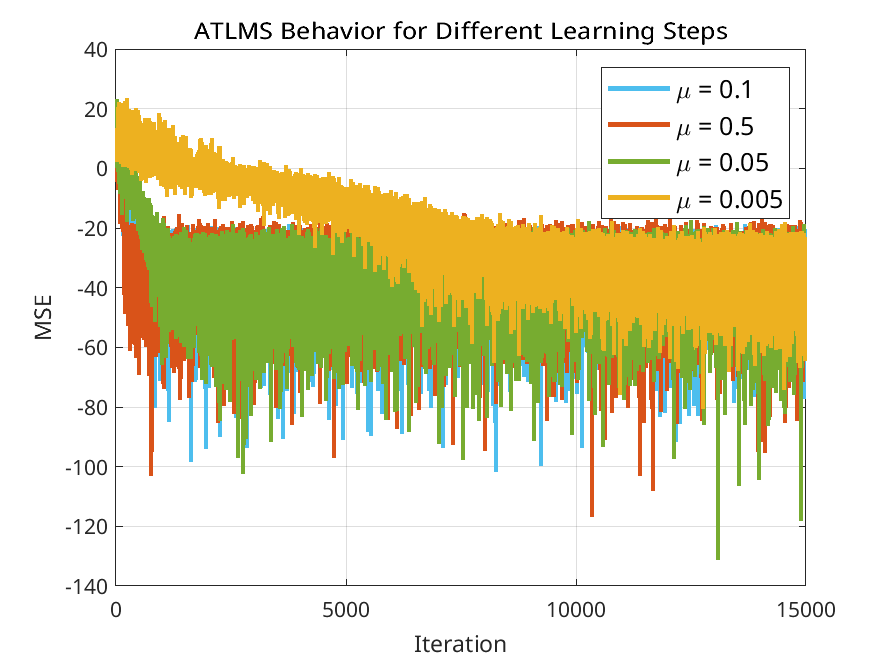
\includegraphics[width=0.90\linewidth]{atlms_mse.png}
        \caption{Monter Carlo Experiment with 2500 runs for LMS algorithm.}
        \label{fig:atlms} 
    \end{figure}
\end{frame}

\begin{frame}
    \frametitle{ATLMS: Different sampling intervals}
    \begin{figure}
        \centering
        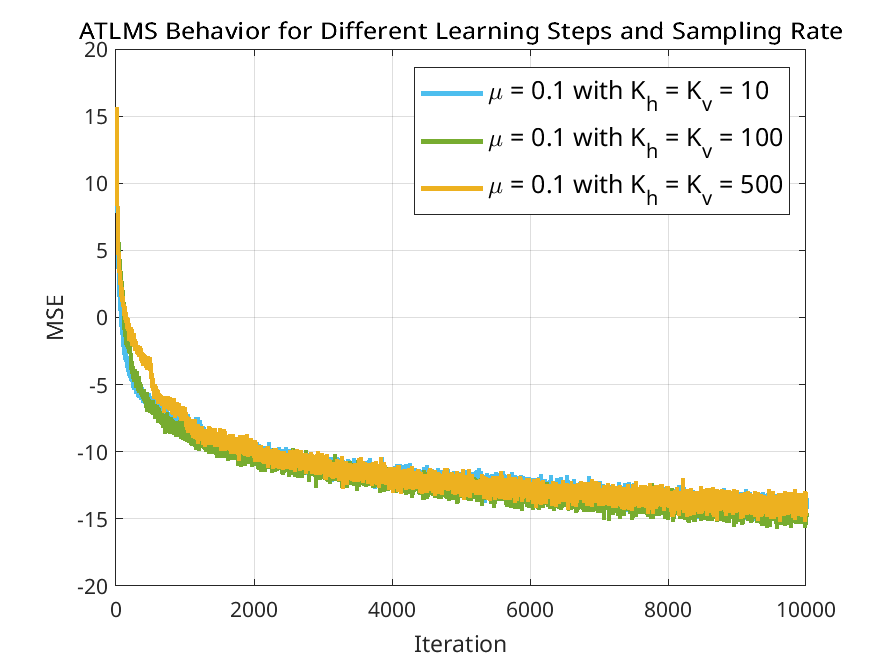
\includegraphics[width=0.90\linewidth]{atlms_sampling.png}
        \caption{Monter Carlo Experiment with 2500 runs for the ATLMS with different sampling intervals.}
        \label{fig:atlms_sampling} 
    \end{figure}
\end{frame}

\begin{frame}
    \frametitle{Processing Time: TLMS vs. ATLMS}
    \begin{figure}
        \centering
        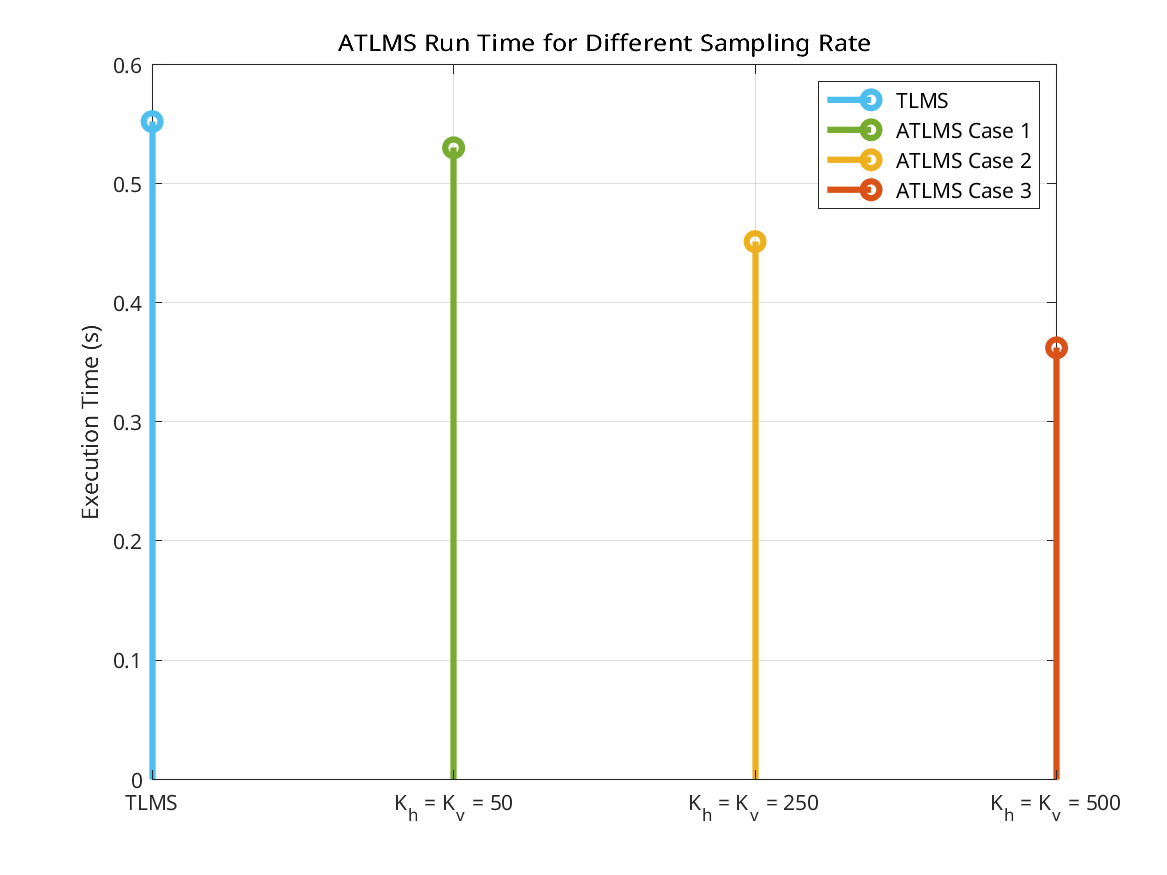
\includegraphics[width=0.90\linewidth]{atlms_time.png}
        \caption{Run time process for ATLMS with different sampling intervals.}
        \label{fig:atlms_time} 
    \end{figure}
\end{frame}

%% Conclusion
\section{Conclusion}
\begin{frame}[allowframebreaks]
    \frametitle{\insertsection}
    \begin{itemize}
        \item TLMS and ATLMS algorithms converges faster than the traditional approachs using NLMS.
        \item TLMS and ATLMS converges to almost the same end, however ATLMS has a greater misadjustment error at the end.
        \item ATLMS can be slightly faster than the TLMS.
    \end{itemize}
\end{frame}

%% References
\section*{References}
\begin{frame} 
    \frametitle{\insertsection}
    \bibliographystyle{ieeetr}
    \bibliography{references}
\end{frame}

%% End of Presentation
\begin{frame}
    \begin{center}
        \Huge Thank you for your presence!
    \end{center}
\end{frame}

\end{document}